\section{CEGIS}
\label{sec:cegis}

\subsection{Motivacija}
\label{subsec:Motivacija}

Program se može sintetisati tako što se definišu njegove specifikacije i zapišu u vidu formule koja se prosledi SMT rešavaču (kao što je na primer Z3). SMT nađe valuaciju koja je zadovoljiva i to predstavlja rešenje. Problem nastaje u tome što formula koja se prosleđuje rezavaču sadrži univerzalne kvantifikatore koje usporavaju pretragu. Naime, rešavač bi u svakom slučaju pronašao rešenje za datu formulu, ali kako bi se to desilo u realnom vremenu, CEGIS (\emph{Counter-Example Guided Inductive Synthesis}) u sebi sadrži posebne taktike za optimizaciju.

Za većinu realnih problema nije neophodno da se razmatraju svi ulazi i izlazi kako bi se došlo do programa koji radi tačno za svaki od njih. Ovako razmišljajući, problem se menja i postaje: \emph{koji je najmanji podskup ulaza koji je potrebno razmatrati da bi se sintetisao program koji zadovoljava date specifikacije?}
CEGIS tehnika upravo traga za tim minimalnim skupom. U petlji, korišćenjem SMT rešavača, on postepeno dolazi do svih mogućih implementacija željenog programa koristeći sve ulaze koji su razmatrani do tog trenutka (počinje sa 0 ulaza). U sledećoj iteraciji on razmatra dalje. Paralelno sa tim, drugim SMT rešavačem pronalazi kontra-primer koji pokazuje da poslednji sintetisani program nije rešenje. Ukoliko kontra-primer ne postoji, poslednji sintetisani prigram je rešenje. Ukoliko se prođe kroz sve iteracije i ne pronađe se rešenje, specifikacija programa nije smislena.

Jedna od mogućih implementacija se može naći na \cite{CEGISimpl}.

\subsection{Arhitektura}
\label{subsec:Arhitektura}

CEGIS se sastoji iz dve faze, induktivne sinteze i verifikacije. Na početku sintezeru dajemo specifikaciju željenog programa. U fazi sinteze pronalazi se program kandidat koji može da zadovolji specifikacije. Nakon toga se u fazi verifikacije proverava da li taj kandidat zaista zadovoljava specifikacije. Ako verifikator ne uspe da pronađe kontra primer znači da smo pronašli traženi program. U suprotnom, verifikator prosleđuje sintezeru informacije o kontra primeru, koje će mu pomoći prilikom daljeg traženja novog kandidata. 

Ovakav vid pretrage zove se pretraga vođena kontra primerima (eng. \emph{counterexample-guided}), zato što je povratna informacija sintezeru kontra primer koji se dodaje u specifikaciju programa. 

Da bismo u potpunosti definisali CEGIS sintezu programa, potrebno je da odgovorimo na nekoliko važnih pitanja:

\begin{itemize}
  \item Kako treba da izgleda specifikacija traženog programa?
  \item Kako ćemo vršiti sintezu programa kandidata?
  \item Kako da proverimo da li program kandidat zadovoljava specifikacije?
  \item Kako da prosledimo povratne informacije za buduće kandidate?
\end{itemize}

staviti ref na ovo zbog slike: https://www.ncbi.nlm.nih.gov/pmc/articles/PMC5597726/


\begin{figure}[h!]
\begin{center}
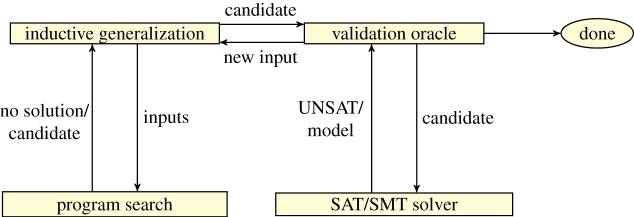
\includegraphics[scale=0.4]{resources/cegis.jpeg}
\end{center}
\caption{CEGIS petlja}
\label{fig:cegis}
\end{figure}


\subsection{Primene CEGISa}
\label{subsec:primeneCEGISa}

Ovo je jedan mogući podnaslov.
